\chapter{经由 \texorpdfstring{$B_{\mathrm{dR}}$}{BdR} 研究 Hasse--Weil \texorpdfstring{$L$}{L} 函数的岩泽理论讲义}
\chapterauthor{加藤和也（Kazuya Kato）}
\begin{center}\large 第一部分\end{center}
\origpage{55}{50}
数学如同夜空，也有两个半球：\term{阿基米德}{archimedean}{archimédien}半球与\term{非阿基米德}{non-archimedean}{non archimédien}半球。由于某些原因，后者通常隐没在我们这个世界的地平线之下，历史上对它的研究也总是落后于前者。

各种 $\zeta$ 函数特殊值的算术，一直是数论的主要课题之一。随着 Tate、Fontaine--Messing、Faltings 等人近来对\term{$p$ 进周期}{$p$-adic periods}{périodes $p$-adiques}理论（即 \term{$p$ 进 Hodge 理论}{$p$-adic Hodge theory}{théorie de Hodge $p$-adique}）的发展，我们如今比以往更能看清 $\zeta$ 值的非阿基米德半球（[BK]、[FP$_1$]、[FP$_2$]、[Ka$_2$] 等）。本文的目的有二：
\begin{itemize}
\item 回顾 $\zeta$ 值与 $p$ 进周期理论之间已知的联系；
\item 说明，在 $\zeta$ 值的非阿基米德半球，我们已经能够看到一个巨大星系的一条旋臂，这个星系就是“\term{$p$ 进 $\zeta$ 元}{$p$-adic zeta elements}{éléments zêta $p$-adiques}”的星系；然而它的全貌仍隐藏在地平线之下。
\end{itemize}
更确切地说，我们预期下述情形成立（第 I 章 §3）：正如所有\term{自守表示}{automorphic representation}{représentation automorphe}都有取值于 $\mathbb C$ 的 $\zeta$ 函数一样，数域上以任意 $p$ 进环 $\Lambda$（它甚至可以是有限环）为系数的所有 \term{Galois 表示}{Galois representation}{représentation galoisienne}，也都有 $p$ 进 $\zeta$ 元；这些元素是某些可逆 $\Lambda$ 模的典范基。由此得到下表，其中 $p$ 进一侧尚属猜想。

\origpage{56}{51}
\begin{center}
\begin{tabular}{>{\raggedright\arraybackslash}p{.43\linewidth}>{\raggedright\arraybackslash}p{.43\linewidth}}\toprule
阿基米德一侧 & $p$ 进一侧\\\midrule
自守表示 & $p$ 进 Galois 表示\\
$\zeta$ 函数 & $p$ 进 $\zeta$ 元\\
$\varepsilon$ 因子 & $\varepsilon$ 元\\
$\cdots$ & $\cdots$\\\bottomrule
\end{tabular}
\end{center}
这两个半球之间的和谐，应当称为广义\term{岩泽理论}{Iwasawa theory}{théorie d'Iwasawa}，或者等价地，称为关于 $\zeta$ 值的广义 Deligne--Beilinson 猜想。对于 Riemann $\zeta$ 函数与 Dirichlet $L$ 函数，岩泽理论是目前研究 $\zeta$ 值算术的最佳理论。倘若能够为 Hasse--Weil $L$ 函数建立岩泽理论，那该多么美好。

$\zeta$ 值的故乡究竟在哪里？在那里，$\zeta$ 值种种天象的真正缘由应当归于何处？我们又怎样才能找到一列驶向故乡的银河列车 [Mi]，以 $p$ 进周期理论为引擎，穿越 $p$ 进 $\zeta$ 元的星系？我想象这列车有一节车厢，名叫“$p$ 进 Galois 表示的\term{显式互反律}{explicit reciprocity law}{loi de réciprocité explicite}”（参见第 II 章 §2 的引言）。

本文（第一部分与第二部分）的结构如下。
\begin{description}
\item[第 I 章] 研究动机与广义岩泽主猜想。\\
§1. 引言，Riemann $\zeta$ 函数。\\
§2. Hasse--Weil $L$ 函数。\\
§3. 广义岩泽主猜想。
\item[第 II 章] 局部理论。\\
§1. $B_{\mathrm{dR}}$ 与相关的 $p$ 进周期理论。\\
§2. Lubin--Tate 群的广义显式互反律。\\
§3.$^{*)}$ 局部主猜想。
\end{description}
\origpage{57}{52}
\begin{description}
\item[第 III 章] 整体问题。\\
§1. 显式互反律与 $\zeta$ 值。\\
§2.$^{*)}$ 动机的 $\zeta$ 值。\\
§3.$^{*)}$ $p$ 进 $L$ 函数与对偶。
\end{description}
第一部分由未标 $^{*)}$ 的各节组成，第二部分则由标有 $^{*)}$ 的各节组成。

各章的内容如下。

第 I 章先回顾关于 $\zeta$ 值的一些已知结果和猜想（§1、§2），再于 §3 提出我们的广义岩泽主猜想。猜想 3.2.2 断言，$p$ 进 Galois 表示的“$p$ 进 $\zeta$ 元”（即复数域中 $\zeta$ 值的非阿基米德对应物）确实存在；对于来自动机的 $p$ 进 Galois 表示，它们与 $\mathbb C$ 中的 $\zeta$ 值满足某种关系（条件 3.2.2(v)）。第 I 章 §3 虽然讨论了条件 3.2.2(v) 的若干重要情形，但其完整表述要到第 III 章 §2 才借助 Fontaine 与 Perrin-Riou 的理论 [FP$_1$][FP$_2$] 给出。猜想 3.2.2 推广了 [BK][FP$_1$][FP$_2$][Ka$_2$] 中关于 $\zeta$ 值的猜想。

我们并未解决这个猜想，而是考察与之有关的若干有趣问题：$\zeta$ 值与显式互反律的关系、$p$ 进 $\zeta$ 元与 $p$ 进 $\zeta$ 函数的关系，等等。这些问题在第 III 章讨论。

第 II 章研究 $p$ 进域的算术与 Fontaine 环 $B_{\mathrm{dR}}$ 的关系。§1 回顾环 $B_{\mathrm{dR}}$，以及相关的 $p$ 进 Galois 表示理论和 $p$ 进周期理论。§2 与 §3 是本文理论上的核心。
\origpage{58}{53}
§2 证明 Lubin--Tate 群的一个广义显式互反律。§3 提出一个称为\term{局部主猜想}{local main conjecture}{conjecture principale locale}的猜想，它是我们的广义岩泽主猜想的局部对应。它断言：$p$ 进局部域上，以 $p$ 进环 $\Lambda$ 为系数的一个 Galois 表示，具有一个 $p$ 进 $\varepsilon$ 元；这个元素是某个 $\Lambda$ 模的基，并且对应于 $\ell$ 进 Galois 表示（$\ell\ne p$）的 $\varepsilon$ 因子。

第 III 章 §1 考察第 II 章 §2 的显式互反律与部分 Riemann $\zeta$ 函数、虚二次域的 Hecke $L$ 级数的值之间的关系，推广 Coates--Wiles 早年对此的研究。§2 回顾 Fontaine 与 Perrin-Riou 的理论 [FP$_1$][FP$_2$]，完成第 I 章 3.2.2 中条件 (v) 的表述。第 III 章 §3 讨论 $p$ 进 $\zeta$ 元与 $p$ 进 $\zeta$ 函数的关系。我们证明，Coates 与 Perrin-Riou 关于 $p$ 进 $L$ 函数的一个猜想 [CP] 可由我们的广义岩泽猜想推出。我们也检验这些猜想与\term{动机}{motive}{motif}的对偶性是否相容。

作者原本希望把本文写成便于初学者阅读的讲义，因此第 I 章 §1 与第 III 章 §1.1 按这一意图写得较为细致。作者喜欢轻松愉快的讲授，所以在第 I 章 3.4.11（谈嘴巴）、第 III 章 1.2.8（谈仙鹤 [Ki]）等处穿插了一些有趣的议论，也写下了开头那段不寻常的引言。不过，限于能力和精力，其他部分恐怕没有那么亲切、那么有趣了：第 I 章的其余部分假定读者熟悉\term{平展上同调}{étale cohomology}{cohomologie étale}，而第 II 章则假定读者熟悉\term{晶体上同调}{crystalline cohomology}{cohomologie cristalline}。

\origpage{59}{54}
作者感谢 S.~Bloch，感谢他将自己引入 $\zeta$ 值这一迷人的领域。他提出的动机 Tamagawa 数的思想 [BK]，是作者研究 $\zeta$ 值的一切工作的基础。作者还感谢 K.~Kimura、N.~Kurokawa、S.~Mochizuki、C.~Nakayama、T.~Saito 和 T.~Uzawa 的建议。

本文约定：对阿贝尔群 $A$ 和整数 $n$，$A/n$ 表示 $A/nA$，而 ${}_nA$ 表示 $\Ker(n\colon A\to A)$。

\section*{第 I 章\quad 研究动机与广义岩泽主猜想}
\addcontentsline{toc}{section}{第 I 章\quad 研究动机与广义岩泽主猜想}
\subsection*{§1. 引言，Riemann $\zeta$ 函数}
\addcontentsline{toc}{subsection}{§1. 引言，Riemann $\zeta$ 函数}
在 §1.1 和 §1.2 中，我设想读者是一位年轻的初学者，试着说明在我看来，$\zeta$ 值究竟有趣在哪里。§1.3 回顾部分 Riemann $\zeta$ 函数的值。

\subsubsection*{§1.1. 认识 $\zeta$ 值的三个阶段}
我认为，我们对 $\zeta$ 函数和 $L$ 函数的值的认识，可以分成三个阶段。下面以 Riemann $\zeta$ 函数
\[
\zeta(s)=\sum_{n\geq1}n^{-s}
\]
为例加以说明。

\origpage{60}{55}
\paragraph{1.1.1. 值的有理性（第一阶段）}
我们首先发现，$\zeta$ 值具有某种“有理性”。Euler 证明了
\begin{align*}
\zeta(2)&=\pi^2/6,\qquad \zeta(4)=\pi^4/90,\qquad\ldots,\tag{1}\\
\zeta(r)\pi^{-r}&\in\mathbb Q\qquad\text{（$r$ 为正偶数）}.\tag{2}
\end{align*}
（关于 Euler 面对这些发现时如何兴奋、如何欣喜，可参见 Weil [We$_2$]。）

Riemann $\zeta$ 函数在 $\operatorname{Re}(s)>1$ 时绝对收敛，经解析延拓成为 $\mathbb C\setminus\{1\}$ 上的全纯函数，并在 $s=1$ 处有一个一阶极点。它满足\term{函数方程}{functional equation}{équation fonctionnelle}
\[
\Lambda(s)=\Lambda(1-s),\qquad
\Lambda(s)=\Gamma(s/2)\pi^{-s/2}\zeta(s).
\]
结合上面的 (2)，得到：
\begin{description}
\item[(3)] 设 $r\leq0$ 为整数，则
\begin{enumerate}[label=(\roman*)]
\item $\zeta(r)\in\mathbb Q$；
\item $\zeta(r)=0$ 当且仅当 $r<0$ 且 $r$ 为偶数。
\end{enumerate}
\end{description}

\paragraph{1.1.2. 值的 $p$ 进性质（第二阶段）}
接下来，我们发现 $\zeta$ 值具有某些 $p$ 进性质。对于 Riemann $\zeta$ 函数，这一点最早由 Kummer 发现。Kubota--Leopoldt 的 $p$ 进 Riemann $\zeta$ 函数理论告诉我们：给定素数 $p$，函数
\[
\{s\in\mathbb Z\mid s\leq0\}\longrightarrow\mathbb Q,
\qquad s\longmapsto(1-p^{-s})\zeta(s)
\]
唯一延拓为连续函数
\[
\left(\varprojlim_n\mathbb Z/p^{n-1}(p-1)\right)\setminus\{1\}
\longrightarrow\mathbb Q_p.
\]
（左端集合以 $\{s\in\mathbb Z\mid s\leq0\}$ 为稠密子集。）

在第一、第二阶段中，我们发现 $\zeta$ 值不仅仅是实、复分析世界中的数，而是属于某个同时超越实、复分析世界和 $p$ 进世界的世界的对象。

\origpage{61}{56}
\paragraph{1.1.3. 值的算术意义（第三阶段）}
第三阶段，我们发现 $\zeta$ 值与算术中一些重要的群有深刻联系，例如\term{理想类群}{ideal class group}{groupe des classes d'idéaux}、\term{Tate--Shafarevich 群}{Tate--Shafarevich group}{groupe de Tate--Shafarevich}等。

Kummer 在这一方向上也是先驱。对 $N\geq1$，令 $\alpha_N=\exp(2\pi i/N)$，并以 $C_N$ 表示 $\mathbb Q(\alpha_N)$ 的理想类群。Kummer 在尝试证明 Fermat 大定理时得到了 Kummer 判别准则：

设 $p$ 为奇素数。则 $p$ 整除 $C_p$ 的阶，当且仅当存在负奇整数 $r$，使 $p$ 整除有理数 $\zeta(r)$ 的分子。

（Kummer 关于 Fermat 大定理的一个结果如下，参见 [Wa] 第 1 章、第 9 章：若 $p$ 是奇素数，且 $p$ 不整除 $C_p$ 的阶，则 Fermat 方程 $x^p+y^p=z^p$ 不存在满足 $x,y,z\in\mathbb Z$ 且 $xyz\ne0$ 的解。）

由 Mazur 与 Wiles [MW] 证明的 Lichtenbaum 猜想，是 Kummer 判别准则的一个精细化：设 $p$ 为奇素数，$r\geq2$ 为偶数，以 $\zeta(1-r)\{p\}$ 表示有理数 $\zeta(1-r)$ 的 $p$ 幂部分，则
\[
\zeta(1-r)\{p\}
=\#H^2(\mathbb Z[1/p],\mathbb Z_p(r))\,
 \#H^1(\mathbb Z[1/p],\mathbb Z_p(r))^{-1}.
\]
这里 $H^*$ 是平展上同调群，$(r)$ 表示 \term{Tate 扭转}{Tate twist}{torsion de Tate}，$\#$ 表示集合的基数。这些平展上同调群都是有限群 [So$_2$]，并且 $q\ne1,2$ 时 $H^q=0$。这个公式与 Kummer 判别准则相联系，因为对任意 $r$，群
\[
H^2(\mathbb Z[1/p],\mathbb Z_p(r))/p
\]
都嵌入 $C_p/p$。

\origpage{62}{57}
经典的分圆域岩泽理论既推广了 Kummer 判别准则，也推广了 Lichtenbaum 猜想；它研究的不只是 $C_N$ 的阶，还包括 $C_N$ 的 $\Gal(\mathbb Q(\alpha_N)/\mathbb Q)$ 模结构（参见 §3.3.9）。

\subsubsection*{§1.2. Hasse--Weil $L$ 函数}
\paragraph{1.2.1.}
数域上簇 $X$ 的 Hasse--Weil $L$ 函数（参见 2.2.3）与 $X$ 的算术性质之间的关系，是数论中一个引人入胜的课题。关于 Hasse--Weil $L$ 函数在整数点处的值，第一、第二阶段已有各种结果与猜想，然而第三阶段我们所知仍然不多。在 §1.2 中，我将说明：人们预期，经典周期理论与 Hasse--Weil $L$ 函数的第一阶段相联系，而 $p$ 进周期理论则与其第二、第三阶段相联系。

\paragraph{1.2.2.}
下面介绍经典周期理论（下述 (1)）与 $p$ 进周期理论（下述 (2)）。

设 $X$ 是域 $K$ 上的光滑固有簇。利用 $X$ 上的微分形式，将 \term{de Rham 上同调}{de Rham cohomology}{cohomologie de de Rham}群 $H^m_{\mathrm{dR}}(X/K)$（$m\in\mathbb Z$）定义为\term{超上同调}{hypercohomology}{hypercohomologie}群 $\mathbb H^m(X,\Omega^\bullet_{X/K})$，其中 $\Omega^\bullet_{X/K}$ 是 de Rham 复形
\[
\bigl[\mathcal O_X\xrightarrow{d}\Omega^1_{X/K}\xrightarrow{d}\cdots\bigr].
\]
对于 $\mathbb C$ 上的光滑概形 $X$，存在典范同构
\[
H^m_{\mathrm{dR}}(X/\mathbb C)\simeq H^m(X(\mathbb C),\mathbb C).\tag{1}
\]
它揭示了微分形式与 \term{Betti 上同调}{Betti cohomology}{cohomologie de Betti}之间的神秘联系。这里 $X(\mathbb C)$ 是赋予经典拓扑的 $X$ 的复点集合。

\origpage{63}{58}
另一方面，设 $X$ 是完备离散赋值域 $K$ 上的光滑概形，$K$ 的剩余域 $k$ 为完美域，且 $\operatorname{char}(K)=0$、$\operatorname{char}(k)=p>0$。近来得到的一个典范同构是
\[
H^m_{\mathrm{dR}}(X/K)\otimes_KB_{\mathrm{dR}}
\simeq H^m_{\mathrm{\acute et}}(X\otimes_K\overline K,\mathbb Q_p)
\otimes_{\mathbb Q_p}B_{\mathrm{dR}}.\tag{2}
\]
它给出了微分形式与 $p$ 进平展上同调之间的神秘联系。这里 $B_{\mathrm{dR}}$ 是 Fontaine [Fo$_1$] 定义的一个大域：无论就其自身规模，还是就它在数学史上的分量而言，都是如此（定义见第 II 章 §1）。同构 (2) 的存在由 Fontaine 在 [Fo$_1$] 中猜测提出，他称之为 \term{de Rham 猜想}{de Rham conjecture}{conjecture de de Rham}；他与 Messing 在一定假设下证明了这一猜想 [Fo$_1$][FM]，Faltings 则证明了其一般情形 [Fa]。

\paragraph{1.2.3.}
现在说明经典同构 1.2.2(1) 如何与 Hasse--Weil $L$ 函数的值相联系。例如，考虑 $\mathbb Q$ 上的\term{椭圆曲线}{elliptic curve}{courbe elliptique}
\[
E=\{(x,y)\mid y^2=x^3+1\}\cup\{\infty\}.
\]
取 $X=E\otimes\mathbb C$、$m=1$，同构 1.2.2(1) 写成
\[
H^1_{\mathrm{dR}}(X/\mathbb C)\xrightarrow{\sim}
H^1(X(\mathbb C),\mathbb C)
=\Hom(H_1(X(\mathbb C),\mathbb Q),\mathbb C),
\]
它将微分形式 $\omega\in H^0(X,\Omega^1_{X/\mathbb C})\subset H^1_{\mathrm{dR}}(X/\mathbb C)$ 映为其上同调类
\[
H_1(X(\mathbb C),\mathbb Q)\longrightarrow\mathbb C,
\qquad \gamma\longmapsto\int_\gamma\omega.
\]
因此，同构 1.2.2(1) 与 $\int_\gamma\omega$ 这样的\term{周期积分}{period integral}{intégrale de période}有关，称为\term{周期同构}{period isomorphism}{isomorphisme des périodes}。类比地，同构 1.2.2(2) 称为 $p$ 进周期同构。

Hasse--Weil $L$ 函数 $L(H^1(E),s)$（参见 2.2.3）的一个值，与某个周期积分有着神秘的联系。令
\origpage{64}{59}
\[
\omega=\frac{dx}{y}\in H^0(E,\Omega^1_{E/\mathbb Q})
\subset H^0(E,\Omega^1_{E/\mathbb Q})\otimes\mathbb C
=H^0(X,\Omega^1_{X/\mathbb C}),
\]
并取 $\gamma$ 为闭路 $E(\mathbb R)$，其方向在 $(x,y)$ 平面中由下向上；将它看作 $H_1(X(\mathbb C),\mathbb Q)$ 的元素。（注意，我们取了一个“有理微分”与一个有理同调类。）那么
\[
L(H^1(E),1)=12^{-1}\int_\gamma\omega.\tag{3}
\]
\begin{center}
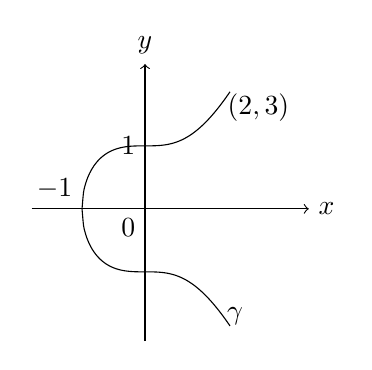
\begin{tikzpicture}[scale=.8]
\draw[->](-1.8,0)--(2.6,0) node[right]{$x$};
\draw[->](0,-2.1)--(0,2.3) node[above]{$y$};
\draw[domain=-1:1.35,samples=100,smooth] plot(\x,{sqrt(\x*\x*\x+1)});
\draw[domain=-1:1.35,samples=100,smooth] plot(\x,{-sqrt(\x*\x*\x+1)});
\node[below left] at(0,0){$0$};\node[above left]at(-1,0){$-1$};
\node[left]at(0,1){$1$};\node[right]at(1.15,-1.7){$\gamma$};
\node at(1.8,1.6){$(2,3)$};
\end{tikzpicture}
\end{center}
（等式 (3) 绝非显然，正如 $\zeta(2)=\pi^2/6$ 也绝非显然一样。）

这种“有理性”推广为 Deligne 的猜想 [De$_3$] 和 Beilinson 的猜想 [Be$_1$][Ra]（参见 §2）。

\paragraph{1.2.4.}
数论中有一个熟知的原则：研究数域上的对象时，局部域上的局部理论起着重要作用。我预期，在 Hasse--Weil $L$ 函数的岩泽理论中（这里固定素数 $p$，研究 $\zeta$ 值与某些重要的 $p$ 进群，例如理想类群的 $p$ 准素部分的关系），$p$ 进局部域上的 $p$ 进周期理论 1.2.2(2) 是最重要的局部理论。简言之，我们预期：$\zeta$ 值通过周期积分理论与微分形式相联系，再通过 $p$ 进周期理论，与平展上同调理论相联系；后者是一种深刻的算术理论，与理想类群、Tate--Shafarevich 群等有关。

\paragraph{1.2.5.}
$p$ 进周期理论仍很年轻，经由 $B_{\mathrm{dR}}$ 来研究 $\zeta$ 值的工作也还不多。然而，重大进展往往发生在两个相距甚远的课题相遇的地方，$B_{\mathrm{dR}}$ 与 $\zeta$ 函数正是这样的两个课题。

\origpage{65}{60}
\subsubsection*{§1.3. Riemann $\zeta$ 函数若干特殊值的回顾}
本节回顾 §1 所说的 Riemann $\zeta$ 函数的第一阶段（定理 1.3.2）和第二阶段（定理 1.3.4、1.3.7）。不过，我们不讨论 $\zeta(3)$、$\zeta(5)$ 等值；这些值与 $K$ 理论有关，参见 §2.2。

\paragraph{1.3.1.}
\term{部分 Riemann $\zeta$ 函数}{partial Riemann zeta function}{fonction zêta partielle de Riemann} $\zeta_{a(N)}(s)$（$a,N\in\mathbb Z$、$N\geq1$）定义为
\[
\zeta_{a(N)}(s)=\sum_{\substack{n\geq1\\n\equiv a\bmod N}}n^{-s}.
\]
函数 $\zeta_{a(N)}(s)$ 在 $\operatorname{Re}(s)>1$ 时绝对收敛，可延拓为 $\mathbb C\setminus\{1\}$ 上的全纯函数，在 $s=1$ 处有一阶极点，留数为 $1/N$。

若 $a\in\mathbb Z/N$，则 $\zeta_{a(N)}(s)$ 指 $\zeta_{b(N)}(s)$，其中 $b$ 为任意满足 $b\bmod N=a$ 的整数。

\begin{statement}{定理 1.3.2}
设 $N\geq1$ 为整数，$a\in\mathbb Z/N$。
\begin{enumerate}[label=(\arabic*)]
\item 对任意整数 $r\leq0$，有 $\zeta_{a(N)}(r)\in\mathbb Q$。
\item 令 $\alpha=\exp(2\pi ia/N)$。则对任意 $r\geq1$，有
\[
(2\pi i)^{-r}\bigl(\zeta_{a(N)}+(-1)^r\zeta_{-a(N)}\bigr)(r)
\in\mathbb Q(\alpha).
\]
若 $\mathbb Q(\alpha)$ 的自同构 $\sigma$ 满足 $\sigma(\alpha)=\alpha^c$，则它将上述元素映为
\[
(2\pi i)^{-r}\bigl(\zeta_{ac(N)}+(-1)^r\zeta_{-ac(N)}\bigr)(r).
\]
\end{enumerate}
\end{statement}
定理 1.3.2 中 $N=1$ 的情形表明：对于偶整数 $r\geq2$，$\zeta(r)\in\mathbb Q\pi^r$；对于整数 $r\leq0$，$\zeta(r)\in\mathbb Q$。

\paragraph{1.3.3.}
固定若干记号。设 $R$ 是 $\mathbb Q$ 上的交换环，$\alpha$ 是 $R$ 中的单位根，$r\leq0$ 为整数。
\begin{enumerate}[label=(\arabic*)]
\item 定义 $\zeta(\alpha,r)\in R$ 为
\[
\zeta(\alpha,r)=\sum_{a\in\mathbb Z/N}\zeta_{a(N)}(r)\alpha^a,
\]
其中 $N\geq1$ 为任意满足 $\alpha^N=1$ 的整数。由 1.3.2(1) 可知 $\zeta_{a(N)}(r)\in\mathbb Q$；所得 $\zeta(\alpha,r)$ 与 $N$ 的选择无关。
\end{enumerate}
\origpage{66}{61}
\begin{enumerate}[label=(\arabic*),start=2]
\item 对素数 $p$，令
\[
\zeta^{(p)}(\alpha,r)=\zeta(\alpha,r)-p^{-r}\zeta(\alpha^p,r)\in R.
\]
\item 对整数 $c\geq1$，令
\[
\zeta_c(\alpha,r)=\zeta(\alpha,r)-c^{1-r}\zeta(\alpha^c,r)\in R.
\]
\item 对分别满足 (2)、(3) 的 $p$、$c$，令
\begin{align*}
\zeta_c^{(p)}(\alpha,r)
&=\zeta^{(p)}(\alpha,r)-c^{1-r}\zeta^{(p)}(\alpha^c,r)\\
&=\zeta_c(\alpha,r)-p^{-r}\zeta_c(\alpha^p,r).
\end{align*}
\end{enumerate}

\begin{statement}{定理 1.3.4}
设 $p$ 为素数，$N\geq1$ 为整数，$c$ 是与 $pN$ 互素的整数。在 (1)、(3)、(4) 中，设 $R$ 为 $\mathbb Q_p$ 上的环，$\alpha\in R$ 是一个 $N$ 次单位根。
\begin{enumerate}[label=(\arabic*)]
\item 对任意整数 $r\leq0$，在 $R$ 中有
\[
\zeta_c(\alpha,r)\in\mathbb Z_{(p)}[\alpha].
\]
这里 $\mathbb Z_{(p)}=\{n/m\mid m,n\in\mathbb Z,\ (p,m)=1\}\subset\mathbb Q$。
\item 设 $r,r'\in\mathbb Z$，$r'\leq r\leq0$。设 $n\geq0$，并假定 $p^n\mid N$。则加法映射
\[
(\mathbb Z/p^n)[t]/(t^N-1)\longrightarrow(\mathbb Z/p^n)[t]/(t^N-1),
\qquad t^a\longmapsto a^{r-r'}t^a
\]
将 $\zeta_c(t,r)\bmod p^n$ 映为 $\zeta_c(t,r')\bmod p^n$。
\item 若 $r,r'\in\mathbb Z$、$r,r'\leq0$，且 $r\equiv r'\bmod(p-1)p^{n-1}$，则
\[
\zeta_c^{(p)}(\alpha,r)\equiv\zeta_c^{(p)}(\alpha,r')
\pmod{p^n\mathbb Z_{(p)}[\alpha]}.
\]
\item 函数
\[
\{r\in\mathbb Z\mid r\leq0\}\longrightarrow\mathbb Z_{(p)}[\alpha],
\quad r\longmapsto\zeta_c^{(p)}(\alpha,r)
\]
唯一延拓为连续函数
\[
\varprojlim_n\mathbb Z/(p-1)p^n\mathbb Z\longrightarrow\mathbb Z_p[\alpha].
\]
相应地，函数
\[
\{r\in\mathbb Z\mid r\leq0\}\longrightarrow\mathbb Q[\alpha],
\quad r\longmapsto\zeta^{(p)}(\alpha,r)
\]
唯一延拓为连续函数
\[
\left(\varprojlim_n\mathbb Z/(p-1)p^n\mathbb Z\right)\setminus\{1\}
\longrightarrow\mathbb Q_p[\alpha].
\]
\end{enumerate}
\end{statement}

\paragraph{1.3.5.}
(1) 设 $R$ 为交换环。对群 $G$，用 $R[G]$ 表示 $G$ 在 $R$ 上的\term{群环}{group ring}{algèbre de groupe}。
\origpage{67}{62}
对\term{投射有限群}{profinite group}{groupe profini} $G$，用 $R[[G]]$ 表示环 $\varprojlim_HR[G/H]$，其中 $H$ 遍历 $G$ 的所有开子群。

(2) 对交换环 $R$，用 $Q(R)$ 表示 $R$ 的\term{全商环}{total quotient ring}{anneau total des fractions}，即 $Q(R)=S^{-1}R$，其中 $S$ 为 $R$ 中所有非零因子组成的集合。

\paragraph{1.3.6.}
对整数 $r\leq0$、$N\geq1$，\term{Stickelberger 元}{Stickelberger element}{élément de Stickelberger} $\theta_N(r)\in\mathbb Q[(\mathbb Z/N)^\times]$ 定义为
\[
\theta_N(r)=\sum_{a\in(\mathbb Z/N)^\times}\zeta_{a(N)}(r)[a]^{-1}.
\]
这里将 $a\in(\mathbb Z/N)^\times$ 视为群环的元素时，记作 $[a]$，以免混淆。

对素数 $p$，令
\[
\theta_{Np^\infty}(r)=\varprojlim_{n\geq1}\theta_{Np^n}(r)
\in\mathbb Q[[(\mathbb Z/Np^\infty)^\times]],
\qquad
(\mathbb Z/Np^\infty)^\times=\varprojlim_n(\mathbb Z/Np^n)^\times.
\]
令
\[
\chi_{\mathrm{cyclo}}\colon(\mathbb Z/Np^\infty)^\times
\longrightarrow\varprojlim_n(\mathbb Z/p^n)^\times
=\mathbb Z_p^\times\subset\mathbb Z_p
\]
为典范映射。

下面的定理可由定理 1.3.4 直接推出。
\begin{statement}{定理 1.3.7}
设 $p$ 为素数，$N\geq1$。
\begin{enumerate}[label=(\arabic*)]
\item 对任意整数 $r\leq0$，$\theta_{Np^\infty}(r)$ 属于全商环
\[Q(\mathbb Z_p[[(\mathbb Z/Np^\infty)^\times]]).\]
更确切地说，对所有
$\sigma\in(\mathbb Z/Np^\infty)^\times$，在
$\mathbb Q_p[[(\mathbb Z/Np^\infty)^\times]]$ 中有
\[
\bigl(1-\chi_{\mathrm{cyclo}}(\sigma)^{1-r}\sigma^{-1}\bigr)
\theta_{Np^\infty}(r)\in\mathbb Z_p[[(\mathbb Z/Np^\infty)^\times]].
\]
\end{enumerate}
\end{statement}
注意，若 $\sigma$ 为无限阶，则 $1-\chi_{\mathrm{cyclo}}(\sigma)^{1-r}\sigma^{-1}$ 是
$\mathbb Z_p[[(\mathbb Z/Np^\infty)^\times]]$ 的非零因子。事实上，此时
$\chi_{\mathrm{cyclo}}(\sigma)^{1-r}$ 不是单位根，而 $\sigma$ 在
$\mathbb Q_p[(\mathbb Z/Np^n)^\times]$ 中的像，对所有 $n\geq0$ 都是单位根。因此
$1-\chi_{\mathrm{cyclo}}(\sigma)^{1-r}\sigma^{-1}$ 在这些环中的像都是非零因子。

\origpage{68}{63}
\begin{statement}{定理 1.3.7（续）}
\begin{enumerate}[label=(\arabic*),start=2]
\item 设 $r,r'\leq0$ 为整数。由
\[
\mathbb Z_p[[(\mathbb Z/Np^\infty)^\times]]
\xrightarrow{\sim}\mathbb Z_p[[(\mathbb Z/Np^\infty)^\times]],
\qquad\sigma\longmapsto\chi_{\mathrm{cyclo}}(\sigma)^{r'-r}\sigma
\]
（$\sigma\in(\mathbb Z/Np^\infty)^\times$）诱导的全商环自同构
\[
Q(\mathbb Z_p[[(\mathbb Z/Np^\infty)^\times]])
\xrightarrow{\sim}Q(\mathbb Z_p[[(\mathbb Z/Np^\infty)^\times]])
\]
将 $\theta_{Np^\infty}(r)$ 映为 $\theta_{Np^\infty}(r')$。
\end{enumerate}
\end{statement}
§1.3 的其余部分给出以上各定理的经典证明。

\paragraph{1.3.8.}
对 $r\geq1$，定义有理函数
\[
g_r(t)\in\mathbb Z[t,(1-t)^{-1}]\subset\mathbb Q(t),
\qquad g_r(t)=-\left(t\frac d{dt}\right)^r\log(1-t).
\]
这里，对任意 $f\in\mathbb Q(t)$ 和 $r\geq1$，符号
$\left(t\frac d{dt}\right)^r\log(f)$ 表示
\[
\left(t\frac d{dt}\right)^{r-1}\left(\frac{f^{-1}df}{t^{-1}dt}\right),
\]
而 $\left(t\frac d{dt}\right)^{r-1}$ 表示算子
\[
t\frac d{dt}\colon\mathbb Q(t)\longrightarrow\mathbb Q(t),
\qquad f\longmapsto t\frac{df}{dt}
\]
的 $r-1$ 次迭代。（定义 $g_r$ 时虽然用了 $\log$ 这个符号，但这里的运算完全是代数的。）有
\begin{align*}
g_1(t)&=t(1-t)^{-1},\quad g_2(t)=t(1-t)^{-2},\quad\ldots,\tag{1}\\
g_r(t)&=\sum_{n\geq1}n^{r-1}t^n\quad\text{在 $\mathbb Q[[t]]$ 中}.\tag{2}
\end{align*}

\paragraph{1.3.9.}
倘若不顾收敛性，就会得到定理 1.3.2、1.3.4、1.3.7 的部分结论的如下“错误证明”。由 1.3.8(2)，有
\[
\zeta(1-r)=\sum_{n\geq1}n^{r-1}=g_r(1).\tag{*}
\]
所以 $\zeta(1-r)$ 是 $\mathbb Q$ 上有理函数 $g_r(t)$ 在 $t=1$ 处的值，因此为有理数。又因为
\[
g_r(t)-p^{r-1}g_r(t^p)=\sum_{\substack{n\geq1\\(n,p)=1}}n^{r-1}t^n,
\]
且当 $(n,p)=1$、$r\equiv r'\bmod(p-1)p^{n-1}$ 时，有
$n^{r-1}\equiv n^{r'-1}\pmod{p^n}$，故
$g_r(t)-p^{r-1}g_r(t^p)\bmod p^n$ 在 $\mathbb Z_p[[t]]$ 中只依赖于
$r\bmod(p-1)p^{n-1}$。
\origpage{69}{64}
这一部分论证是正确的。因此，若忽略收敛性，令 $t=1$，便得到
$\zeta^{(p)}(r)\bmod p^n$ 只依赖于 $r\bmod(p-1)p^{n-1}$。

这些错误证明实际上“几乎正确”；下面只需修改这些论证，就能得到各定理的真正证明。

\begin{statement}{引理 1.3.10}
设 $r,c\in\mathbb Z$，$r\geq1$、$c\ne0$，令
\[
g_{r,c}(t)=g_r(t)-c^rg_r(t^c)\in\mathbb Q(t).
\]
设 $N\geq1$ 为整数，$(c,N)=1$，则 $g_{r,c}(t)$ 在所有 $N$ 次单位根处均无极点。
\end{statement}
\begin{proof}
由
\[
g_{r,c}(t)=\left(t\frac d{dt}\right)^r
\log\bigl((1-t^c)(1-t)^{-1}\bigr)
\]
以及 $(1-t^c)(1-t)^{-1}$ 在 $N$ 次单位根处既无零点也无极点，即得结论。
\end{proof}

\begin{statement}{引理 1.3.11}
对整数 $c\ne0$，令
\[
R_c=\mathbb Z[t^{\pm1},\{(1-t^c)(1-t)^{-1}\}^{\pm1}].
\]
\begin{enumerate}[label=(\arabic*)]
\item $g_{r,c}(t)\in R_c$。
\item 设 $N\geq1$ 为整数，$(c,N)=1$。则 $R_c$ 在
$\mathbb Q[t]/(t^N-1)$ 中的像包含于 $\mathbb Z[1/c,t]/(t^N-1)$。
特别地，由 (1)，$g_{r,c}(t)$ 在 $\mathbb Q[t]/(t^N-1)$ 中的像也包含于
$\mathbb Z[1/c,t]/(t^N-1)$。
\end{enumerate}
\end{statement}
\begin{proof}
(1) 由 1.3.10 证明中 $g_{r,c}(t)$ 的表达式即得。

对 $c$ 与 $-c$，断言 (2) 等价，因此可以假设 $c>0$。只需证明
$(1-t^c)(1-t)^{-1}$ 在 $\mathbb Z[1/c,t]/(t^N-1)$ 中可逆。
\origpage{70}{65}
设 $I$ 为 $\mathbb Z[t]$ 中由 $(1-t^c)(1-t)^{-1}$ 与 $1-t^N$ 生成的理想，只需证明 $c\in I$。由于 $t^c\equiv t^N\equiv1\pmod I$，有 $t\equiv1\pmod I$，从而 $1-t\in I$。又
$(1-t^c)(1-t)^{-1}\equiv c\pmod{1-t}$，故 $c\in I$，得证。
\end{proof}

\paragraph{1.3.12.}
现在开始分析方面的论证。对 $(t,s)\in\mathbb C\times\mathbb C$，若满足
$|t|\leq1$ 且 $\operatorname{Re}(s)>1$，或者满足 $|t|<1$，定义
\[
\zeta(t,s)=\sum_{n\geq1}t^nn^{-s}.
\]
此级数绝对收敛。下面的引理留待 1.3.20 证明。

\begin{statement}{引理 1.3.13}
令 $F=\{t\in\mathbb R\mid t\geq1\}$。
\begin{enumerate}[label=(\arabic*)]
\item $\zeta(t,s)$ 可延拓为 $(\mathbb C\setminus F)\times\mathbb C$ 上的全纯函数。
\item 对任意整数 $c\geq1$，关于 $(t,s)$ 的函数
\[
\zeta_c(t,s)\mathrel{\mathop:}=\zeta(t,s)-c^{1-s}\zeta(t^c,s)
\]
可延拓为
\[
\bigl(\mathbb C\setminus\{t\in\mathbb C\mid t\notin F,\ t^c\in F\}\bigr)\times\mathbb C
\]
上的全纯函数。
\end{enumerate}
\end{statement}

\begin{statement}{推论 1.3.14}
\begin{enumerate}[label=(\arabic*)]
\item 若 $\alpha$ 是 $\mathbb C$ 中的单位根，且 $\alpha\ne1$，则 $s\longmapsto\zeta(\alpha,s)$ 可延拓为 $\mathbb C$ 上的全纯函数。
\item 若 $\alpha$ 是 $\mathbb C$ 中的单位根，而整数 $c\geq1$ 与 $\alpha$ 的阶 $N$ 互素，则 $s\longmapsto\zeta_c(\alpha,s)$ 可延拓为 $\mathbb C$ 上的全纯函数。
\item 作为 (2) 的特殊情形，对任意整数 $c\geq1$，映射
\[
s\longmapsto\zeta_c(1,s)=(1-c^{1-s})\zeta(s)
\]
可延拓为 $\mathbb C$ 上的全纯函数。
\end{enumerate}
\end{statement}
由 1.3.14，以及当 $\alpha$ 为 $N$ 阶单位根时成立的等式
\[
\zeta(\alpha,s)=\sum_{a\in\mathbb Z/N}\zeta_{a(N)}(s)\alpha^a,
\]
容易看出，$\zeta_{a(N)}(s)$ 可以延拓为 $\mathbb C$ 上的亚纯函数，并在 $s\ne1$ 处全纯。

\origpage{71}{66}
\begin{statement}{引理 1.3.15}
\begin{enumerate}[label=(\arabic*)]
\item 对任意整数 $r\geq1$ 及任意 $t\in\mathbb C\setminus F$，有
$g_r(t)=\zeta(t,1-r)$。
\item 设 $c\geq1$ 为整数。则对任意整数 $r\geq1$ 及任意
$t\in\mathbb C\setminus\{t\in\mathbb C\mid t\notin F,\ t^c\in F\}$，有
$g_{r,c}(t)=\zeta_c(t,1-r)$。
\end{enumerate}
\end{statement}
\begin{proof}
这些等式在 $|t|<1$ 时成立，故在上述范围内均成立。
\end{proof}

\begin{statement}{推论 1.3.16}
设 $c,N\geq1$ 为整数，$(c,N)=1$。以
\[
\sigma_c\colon\mathbb C[t]/(t^N-1)\longrightarrow\mathbb C[t]/(t^N-1)
\]
表示由 $t\longmapsto t^c$ 给出的 $\mathbb C$ 代数同态。则对于整数 $r\geq1$，元素
\[
\sum_{a\in\mathbb Z/N}\zeta_{a(N)}(1-r)t^a
\]
在映射
\[
1-c^r\sigma_c\colon\mathbb C[t]/(t^N-1)\longrightarrow\mathbb C[t]/(t^N-1)
\]
下的像恰为 $g_{r,c}(t)\bmod(t^N-1)$。
\end{statement}

\paragraph{1.3.17.}
证明定理 1.3.2(1)。设 $r,N\geq1$ 为整数，取与 $N$ 互素的整数 $c$。由 1.3.16，
$\sum_{a\in\mathbb Z/N}\zeta_{a(N)}(1-r)t^a$ 在
$1-c^r\sigma_c\colon\mathbb C[t]/(t^N-1)\to\mathbb C[t]/(t^N-1)$ 下的像属于
$\mathbb Q[t]/(t^N-1)$。再取 $c\geq2$，则 $1-c^r\sigma_c$ 为双射，并诱导双射
$\mathbb Q[t]/(t^N-1)\xrightarrow{\sim}\mathbb Q[t]/(t^N-1)$。这就证明了
\[
\sum_{a\in\mathbb Z/N}\zeta_{a(N)}(1-r)t^a\in\mathbb Q[t]/(t^N-1).
\]

\paragraph{1.3.18.}
利用部分 Riemann $\zeta$ 函数在正整数与负整数处的值之间的下述关系，可由 1.3.2(1) 推出 1.3.2(2)。（第 III 章 §1.1 给出 1.3.2(2) 的另一个证明，不使用负整数处的值。）

设 $a,N\in\mathbb Z$、$N\geq1$，令 $\alpha=\exp(2\pi ia/N)$。设 $r\in\mathbb Z$；若 $r=0$，再假定 $\alpha\ne1$，则
\origpage{72}{67}
\begin{align*}
&\frac12\bigl(\zeta(\alpha,1-r)+(-1)^r\zeta(\alpha^{-1},1-r)\bigr)\\
&\qquad=\left(\frac{-2\pi i}{N}\right)^{-r}
\lim_{s\to r}\Gamma(s)\bigl(\zeta_{a(N)}(s)+(-1)^r\zeta_{-a(N)}(s)\bigr).
\end{align*}
当 $r\geq2$ 时，左端等于 $\zeta(\alpha,1-r)$。

这可由 Dirichlet $L$ 级数的函数方程推出（[Wa] 第 4 章）。

\paragraph{1.3.19.}
证明定理 1.3.4。我们已经得到
\[
\zeta_c(t,1-r)=g_{r,c}(t)\qquad\text{在 $\mathbb Q[t]/(t^N-1)$ 中}.\tag{*}
\]
1.3.4(1) 由 (*) 和 1.3.11 推出；1.3.4(2) 由 (*) 以及
$\left(t\frac d{dt}\right)g_r=g_{r+1}$ 推出。为证明 1.3.4(3)，以 $Np^n$ 代替 $N$，可假定 $p^n\mid N$。于是，由 1.3.4(2)、等式
$\left(t\frac d{dt}\right)^r(t^a)=a^rt^a$（$r\geq0$），以及下述初等事实，即得 1.3.4(3)：若 $a\in\mathbb Z_p^\times$，且
$r\equiv0\bmod(p-1)p^{n-1}$，则 $a^r\equiv1\pmod{p^n}$。最后，1.3.4(4) 由 1.3.4(3) 推出。

\paragraph{1.3.20.}
证明 1.3.13。取 $F$ 如 1.3.13 中所定。对
$(t,s)\in(\mathbb C\setminus F)\times\mathbb C$，令
\[
H(t,s)=(2\pi i)^{-1}\int_\gamma
(1-\exp(x)t)^{-1}\exp(x)t\,x^s x^{-1}\,dx,\tag{1}
\]
其中 $\gamma$ 是复平面中如下所示的路径。
\begin{center}
\begin{tikzpicture}[scale=.85]
\draw[->](-4,0)--(2.4,0)node[right]{$\mathbb R$};
\draw[->,dashed](0,-1.15)--(0,1.4)node[above]{$\mathbb R i$};
\draw(-3.8,-.25)--(.12,-.25) arc(-90:90:.25) --(-3.8,.25);
\foreach \x in {-3.2,-2.4,-1.6,-.8}{\draw[->](\x-.25,-.25)--(\x+.2,-.25);\draw[->](\x+.2,.25)--(\x-.25,.25);}
\node[right]at(.38,0){$\gamma$};
\end{tikzpicture}
\end{center}
这里 $x^s$ 定义为 $\exp(s\log(x))$，$\log$ 取
$\mathbb C\setminus\{x\in\mathbb R\mid x\leq0\}$ 上的主支。对每个 $(t,s)$，路径 $\gamma$ 都取在足够靠近
$\{x\in\mathbb R\mid x\leq0\}$ 的地方，使关于 $x$ 的函数 $1-\exp(x)t$ 在 $\gamma$ 上及其所围区域内均无零点。

于是，$H(t,s)$ 是 $(\mathbb C\setminus F)\times\mathbb C$ 上的全纯函数。

\begin{statement}{引理 1.3.21}
\begin{enumerate}[label=(\arabic*)]
\item 若 $|t|\leq1$、$t\ne1$ 且 $\operatorname{Re}(s)>1$，则
$\zeta(t,s)=\Gamma(1-s)H(t,s)$。
\item 对任意整数 $c\geq1$，$H(t,s)-c^{1-s}H(t^c,s)$ 可延拓为
$\mathbb C\times\mathbb C$ 中 $F\times\mathbb C$ 的某个邻域上的全纯函数。
\end{enumerate}
\end{statement}
\origpage{73}{68}
\begin{proof}[（1）的证明]
若 $|t|\leq1$、$t\ne1$ 且 $\operatorname{Re}(s)>1$，则
\begin{align*}
H(t,s)
&=(2\pi i)^{-1}\int_{-\infty}^{0}
 (1-\exp(x)t)^{-1}\exp(x)t(-x)^s\exp(-\pi is)x^{-1}\,dx\\
&\quad +(2\pi i)^{-1}\int_{0}^{-\infty}
 (1-\exp(x)t)^{-1}\exp(x)t(-x)^s\exp(\pi is)x^{-1}\,dx\\
&=(2\pi i)^{-1}\bigl(\exp(\pi is)-\exp(-\pi is)\bigr)
 \int_0^\infty(1-\exp(-y)t)^{-1}\exp(-y)t\,y^s y^{-1}\,dy\\
&=(2\pi i)^{-1}\bigl(\exp(\pi is)-\exp(-\pi is)\bigr)
 \sum_{n\geq1}\int_0^\infty\exp(-ny)t^n y^s y^{-1}\,dy\\
&=(2\pi i)^{-1}\bigl(\exp(\pi is)-\exp(-\pi is)\bigr)
 \Gamma(s)\sum_{n\geq1}t^nn^{-s}\\
&=\Gamma(1-s)^{-1}\zeta(t,s).
\end{align*}
因此，$\zeta(t,s)$ 可延拓为 $(\mathbb C\setminus F)\times\mathbb C$ 上的亚纯函数。下面证明它实际上全纯。此函数的极点除子包含于 $\Gamma(1-s)$ 的极点除子
\[
(\mathbb C\setminus F)\times\{r\in\mathbb Z\mid r\geq1\}.
\]
但 $\zeta(t,s)$ 在 $\{t\in\mathbb C\mid |t|<1\}\times\mathbb C$ 上没有极点，故它处处无极点。
\end{proof}
\begin{proof}[（2）的证明]
在积分式 1.3.20(1) 中，以 $t^c$ 代替 $t$、$cx$ 代替 $x$，得到
\[
c^{1-s}H(t^c,s)=(2\pi i)^{-1}\int_\gamma
c(1-\exp(cx)t^c)^{-1}\exp(cx)t^c x^s x^{-1}\,dx.
\]
若 $t\in\mathbb C\setminus\{t\in\mathbb C\mid t\notin F,\ t^c\in F\}$，则关于 $x$ 的函数
\[
(1-\exp(x)t)^{-1}-c(1-\exp(cx)t^c)^{-1}
\]
在 $\{x\in\mathbb R\mid x\leq0\}$ 的某个邻域上全纯。
\end{proof}

\subsection*{§2. Hasse--Weil $L$ 函数}
\addcontentsline{toc}{subsection}{§2. Hasse--Weil $L$ 函数}
本节在介绍\term{行列式模}{determinant module}{module déterminant}的预备知识（§2.1）之后，回顾一些特殊情形下，关于 Hasse--Weil $\zeta$ 函数在整数点处的值的第一、第三阶段（按 §1.1 的意义）的猜想。
\origpage{74}{69}
如果 Hasse--Weil $L$ 函数在所考虑的整数点处有零点或极点，我们关心的是它在该点的 Laurent 展开中首个非零系数，也把这个系数称为“$\zeta$ 值”。第一阶段由著名的 Beilinson 猜想 [Be$_1$][Ra] 表述：模去 $\mathbb Q^\times$，$\zeta$ 值可用 $K$ 理论的\term{调节映射}{regulator map}{application régulateur}与周期积分表示。为简化回顾，本节只考虑两个极端情形：出现 $K$ 理论而不出现周期积分的情形（§2.2），以及出现周期积分而不出现 $K$ 理论的情形，后者称为\term{临界情形}{critical case}{cas critique}（§2.3）。在临界情形，Beilinson 猜想归结为 Deligne 早先提出的猜想 [De$_3$]。实际上，为进一步简化叙述，§2.3 只讨论 Birch--Swinnerton-Dyer 猜想的一个特殊情形。在 §2.2（分别地，§2.3）所考虑的情形下，[BK][FP$_1$][FP$_2$][Ka$_2$] 中关于 Hasse--Weil $L$ 函数第三阶段的猜想断言，$\zeta$ 值通过 $K$ 理论中的 \term{Chern 类映射}{Chern class map}{application des classes de Chern}（分别地，通过 $p$ 进周期理论），与平展上同调发生如下联系：
\[
\begin{tikzcd}[ampersand replacement=\&,column sep=huge,row sep=large]
\text{$\zeta$ 值}\arrow[r,dash,"{\text{调节映射}}"]\arrow[d,dash,"{\text{周期积分}}"']
\&\text{$K$ 理论}\arrow[d,dash,"{\text{Chern 类映射}}"]\\
\text{微分形式}\arrow[r,dash,"{\text{$p$ 进周期}}"]\&\text{平展上同调}
\end{tikzcd}
\]
这些猜想将包含在 §3 的广义岩泽主猜想之中（参见 2.3.5）。本节不讨论这些结果的证明。

\origpage{75}{70}
\subsubsection*{§2.1. 行列式模}
这里对行列式模作若干说明。§2.1 中，$\Lambda$ 表示交换环。

\paragraph{2.1.1.}
$\Lambda$ 上的\term{完美复形}{perfect complex}{complexe parfait}，指 $\Lambda$ 模的\term{导出范畴}{derived category}{catégorie dérivée}中的一个对象，它可由有界复形
\[
(\cdots\longrightarrow P^q\longrightarrow P^{q+1}\longrightarrow\cdots)
\]
表示，其中每个 $P^q$ 都是有限生成投射 $\Lambda$ 模。

\paragraph{2.1.2.}
考虑如下三个范畴 $\mathscr L$、$\mathscr C$、$\mathscr E$。
$\mathscr L$ 的对象是二元组 $(L,r)$，其中 $L$ 是可逆 $\Lambda$ 模，$r$ 是局部常值函数
$\Spec(\Lambda)\to\mathbb Z$。当 $r=r'$ 时，态射 $(P,r)\to(P',r')$ 为同构 $P\xrightarrow{\sim}P'$；当 $r\ne r'$ 时，不存在这样的态射。
$\mathscr C$ 的对象为 $\Lambda$ 上的完美复形（2.1.1）；$\mathscr E$ 的对象为 $\Lambda$ 模复形的正合列
\[
0\longrightarrow F'^\bullet\longrightarrow F^\bullet
\longrightarrow F''^\bullet\longrightarrow0,
\]
其中各复形视为导出范畴的对象时都是完美的。这里它们确实是复形，而非仅仅导出范畴的对象。$\mathscr C$ 与 $\mathscr E$ 中的态射均为显然意义下的同构。

Knudsen 与 Mumford 在 [KM] 中证明：存在一对 $(\det_\Lambda,i)$，在典范同构意义下唯一，其中
$\det_\Lambda\colon\mathscr C\to\mathscr L$ 为函子，而 $i\colon f\xrightarrow{\sim}g$ 为同构；这里 $f,g\colon\mathscr E\to\mathscr L$ 定义为
\begin{align*}
f(0\to F'^\bullet\to F^\bullet\to F''^\bullet\to0)
 &=\det_\Lambda(\widetilde F^\bullet),\\
g(0\to F'^\bullet\to F^\bullet\to F''^\bullet\to0)
 &=\det_\Lambda(\widetilde F'^\bullet)\otimes_\Lambda
   \det_\Lambda(\widetilde F''^\bullet),
\end{align*}
并且满足某些条件。这里 $\widetilde F^\bullet$ 等表示由 $F^\bullet$ 等对应的导出范畴对象，
$\otimes_\Lambda$ 表示函子 $\mathscr L\times\mathscr L\to\mathscr L$，由
\[
(L,r)\otimes_\Lambda(L',r')=(L\otimes_\Lambda L',r+r')
\]
给出。
\origpage{76}{71}
上述“某些条件”包括下面两个条件。
\begin{enumerate}[label=(\roman*)]
\item 对有限生成投射 $\Lambda$ 模 $P$，将它视为集中在次数 $0$ 的导出范畴对象时，
$\det_\Lambda(P)$ 为如下定义的二元组 $(L,r)$：令 $\widetilde P$ 为 $\Spec(\Lambda)$ 上与 $P$ 对应的拟凝聚层，它是有限秩局部自由层；则 $r$ 为 $\widetilde P$ 的秩，而 $L$ 为对应于 $\widetilde P$ 的第 $r$ 次外幂的 $\Lambda$ 模。
\item 对 $\mathscr E$ 的对象
$E=(0\to P'\to P\xrightarrow{\pi}P''\to0)$，其中 $P,P',P''$ 为有限生成投射 $\Lambda$ 模，视为集中在次数 $0$ 的复形，同构 $i_E$ 在 $\Spec(\Lambda)$ 上由下式局部刻画：
\[
x_1\wedge\cdots\wedge x_r\longmapsto
(x_1\wedge\cdots\wedge x_{r'})\otimes
\bigl(\pi(x_{r'+1})\wedge\cdots\wedge\pi(x_r)\bigr).
\]
这里 $r,r',r''$ 分别为 $P,P',P''$ 的秩\footnote{译注：原书此句给出的 $P$ 与 $P'$ 次序和上方外积公式不一致；这里依公式明确两者的对应。}，
$x_1,\ldots,x_{r'}$ 为 $\widetilde P'$ 的局部截面，
$x_{r'+1},\ldots,x_r$ 为 $\widetilde P$ 的局部截面。
\end{enumerate}

\paragraph{2.1.3.}
固定 2.1.2 中的一对 $(\det_\Lambda,i)$。本文稍作记号变更：将原来的 $\det_\Lambda$ 忘掉二元组 $(L,r)$ 中的 $r$ 后，所得从 $\mathscr C$ 到可逆 $\Lambda$ 模范畴的函子，仍记为 $\det_\Lambda$。

设 $\mathscr C$ 中的对象 $C$ 由 2.1.1 所述的有界复形表示，则有典范同构
\[
\det_\Lambda(C)\simeq\bigotimes_{q\in\mathbb Z}
\{\det_\Lambda(P^q)\}^{(-1)^q}.
\]
若上同调模 $H^q(C)$ 视为集中在次数 $0$ 的导出范畴对象时均为完美的，则有典范同构
\[
\det_\Lambda(C)\simeq\bigotimes_{q\in\mathbb Z}
\{\det_\Lambda(H^q(C))\}^{(-1)^q}
\]
（[KM] 定理 2 后的注 b)）。

\origpage{77}{72}
处理这些行列式模时应当小心，因为某些典范同构稍不留意就会多出一个 $-1$ 的因子。不过，遇到这种微妙情形时，本文只在相差一个符号的意义下讨论，因此这一点在这里并不构成严重问题。（我希望本文中的符号不确定性将来能够消除。）

\paragraph{2.1.4.}
设 $\Lambda$ 是正则 Noether 环，$F$ 是有限生成 $\Lambda$ 模，则 $F$ 有一个由有限生成投射 $\Lambda$ 模组成的有限消解。因此，将 $F$ 视为集中在次数 $0$ 的导出范畴对象时，它是完美复形，故 $\det_\Lambda(F)$ 有定义。

以 $Q(\Lambda)$ 表示 $\Lambda$ 的全商环，假设 $F\otimes_\Lambda Q(\Lambda)=0$，即 $F$ 为挠 $\Lambda$ 模。令
$\operatorname{char}_\Lambda(F)$ 为由下述性质刻画的可逆理想：对 $\Lambda$ 的每个高度为一的素理想 $\mathfrak p$，
\[
\operatorname{char}_\Lambda(F)_{\mathfrak p}
=(\mathfrak p\Lambda_{\mathfrak p})^n,
\qquad n=\operatorname{length}_{\Lambda_{\mathfrak p}}(F_{\mathfrak p}).
\]

\begin{statement}{2.1.5（[KM] 定理 3(vi)）}
设 $\Lambda$ 为正则 Noether 环，$F$ 为有限生成挠 $\Lambda$ 模。沿用上述记号，复合单同态
\begin{align*}
\det_\Lambda(F)&\lhook\joinrel\longrightarrow
\det_\Lambda(F)\otimes_\Lambda Q(\Lambda)\\
&\xrightarrow{\sim}\det_{Q(\Lambda)}(F\otimes_\Lambda Q(\Lambda))
=\det_{Q(\Lambda)}([0])=Q(\Lambda)
\end{align*}
的像，恰为分式理想 $\operatorname{char}_\Lambda(F)^{-1}$。
\end{statement}
\begin{proof}
将 $\Lambda$ 换为其在高度为一的素理想 $\mathfrak p$ 处的局部环 $\Lambda_{\mathfrak p}$，可假设 $\Lambda$ 是离散赋值环。进而可假定 $F=\Lambda/a\Lambda$，其中 $a\in\Lambda$ 为非零元。于是，在导出范畴中
\[
\Lambda/a\Lambda\simeq
\bigl(\underbrace{a\Lambda}_{\text{次数 }-1}
\longrightarrow\underbrace{\Lambda}_{\text{次数 }0}\bigr),
\]
故在其与 $Q(\Lambda)$ 的张量积中，有
\[
\det_\Lambda(\Lambda/a\Lambda)
=\Lambda\otimes_\Lambda(a\Lambda)^{-1}=a^{-1}\Lambda.
\]
\end{proof}

\origpage{78}{73}
\subsubsection*{§2.2. $K$ 理论与 $\zeta$ 值}
\paragraph{2.2.1.}
对任意概形 $X$，Quillen 的 $K$ 群 $K_n(X)$（$n\geq0$）都有定义 [Qu]。若
$X=\Spec(\mathcal O_K)$，其中 $\mathcal O_K$ 为数域 $K$ 的整数环，则
\[
K_0(X)\simeq\mathbb Z\oplus\Pic(\mathcal O_K),
\qquad K_1(X)\simeq\mathcal O_K^\times.
\]
理想类群 $\Pic(\mathcal O_K)$ 与\term{单位群}{unit group}{groupe des unités} $\mathcal O_K^\times$ 在数论中居于核心地位，因此自然会预期高阶 $K$ 群 $K_n$ 同样重要。今天，我们已经知道事实确实如此。

在 §2.2 中，我们首先回顾 $\mathcal O_K^\times$ 上的调节映射与 Dedekind $\zeta$ 函数在 $s=0$ 处的性质之间的经典联系，再回顾关于 Hasse--Weil $L$ 函数值的第一阶段（著名的 Beilinson 猜想）与第三阶段（[BK][FP$_1$][FP$_2$][Ka$_2$] 中的猜想；我们采用 [FP$_1$][FP$_2$] 的表述）中已有猜想的一个特殊情形。这里考虑的情形既不出现周期积分，也不出现 $p$ 进周期，仅凭 $K$ 理论便足以在猜想层面上，将 $\zeta$ 值与平展上同调联系起来。

\paragraph{2.2.2.}
回顾经典调节子理论中，单位群与理想类群如何同 Dedekind $\zeta$ 函数相联系。有实向量空间的同构
\[
(\log\|\ \|_v)_v\colon\mathcal O_K^\times\otimes\mathbb R
\xrightarrow{\sim}\left(\bigoplus_v\mathbb R\right)^0,\tag{1}
\]
其中 $v$ 遍历 $K$ 的所有阿基米德素位，
\[
\left(\bigoplus_v\mathbb R\right)^0
=\left\{(a_v)_v\in\bigoplus_v\mathbb R\ \middle|\ \sum_va_v=0\right\},
\]
$\|\ \|_v$ 是素位 $v$ 处的归一化绝对值。称为 $K$ 的\term{调节子}{regulator}{régulateur}的正实数 $R_K$，定义为
$\mathcal O_K^\times$ 在 $(\bigoplus_v\mathbb R)^0$ 中的像，相对于格
$(\bigoplus_v\mathbb Z)^0$ 的体积。

\origpage{79}{74}
有
\[
\lim_{s\to0}s^{-e}\zeta_K(s)=-\frac{R_Kh_K}{w_K},\tag{2}
\]
其中 $\zeta_K(s)$ 为 $K$ 的 \term{Dedekind $\zeta$ 函数}{Dedekind zeta function}{fonction zêta de Dedekind}，
$e=r_1+r_2-1$，$r_1$、$r_2$ 分别是 $K$ 的实素位、复素位的个数，
$h_K=\#\Pic(\mathcal O_K)$ 为 $K$ 的\term{类数}{class number}{nombre de classes}，
$w_K$ 为 $K$ 中单位根的个数。

性质
\[
R_K^{-1}\lim_{s\to0}s^{-e}\zeta_K(s)\in\mathbb Q
\]
是 $\zeta_K(s)$ 在 $s=0$ 处性质的第一阶段，而公式 (2) 是第三阶段。

注意，忽略符号，公式 (2) 可以用行列式模改述如下：存在元素
$z\in\det_{\mathbb Q}(\mathcal O_K^\times\otimes\mathbb Q)$，它在由 (1) 诱导的映射
\[
\det_{\mathbb Q}(\mathcal O_K^\times\otimes\mathbb Q)\otimes\mathbb R
\xrightarrow{\sim}
\det_{\mathbb Z}\left(\left(\bigoplus_v\mathbb Z\right)^0\right)\otimes\mathbb R
\]
下，映为 $\lim_{s\to0}s^{-e}\zeta_K(s)$ 乘以
$\det_{\mathbb Z}((\bigoplus_v\mathbb Z)^0)$ 的某个 $\mathbb Z$ 基（这就是第一阶段的部分），并且
\[
[\det_{\mathbb Z}(\mathcal O_K^\times):\mathbb Zz]=h_K.\tag{3}
\]
这里 $\det_{\mathbb Z}(\mathcal O_K^\times)$ 与 $\mathbb Zz$ 都视为一维 $\mathbb Q$ 向量空间
$\det_{\mathbb Q}(\mathcal O_K^\times\otimes\mathbb Q)$ 中的 $\mathbb Z$ 格。对于两个这样的格 $L,L'$，定义
\[
[L:L']=\#(L/L'')\,\#(L'/L'')^{-1},\qquad L''=L\cap L'.
\]

\paragraph{2.2.3.}
现在考虑 Hasse--Weil $L$ 函数。首先回顾 $p$ 进 Galois 表示的 $L$ 函数。

令 $\overline{\mathbb Q}$ 为 $\mathbb Q$ 的一个代数闭包。考虑四元组 $(p,S,V,A)$，其中：
\begin{itemize}
\item $p$ 为素数；
\item $S$ 为包含 $p$ 的有限素数集；
\end{itemize}
\origpage{80}{75}
\begin{itemize}
\item $V$ 为有限维 $\mathbb Q_p$ 向量空间，带有在 $S$ 外非分歧的连续
$\Gal(\overline{\mathbb Q}/\mathbb Q)$ 作用；
\item $A$ 是 $\mathbb Q$ 上的交换环，为 $\mathbb Q$ 的有限扩张的有限直积，并且作用于 $V$，该作用与
$\Gal(\overline{\mathbb Q}/\mathbb Q)$ 的作用交换。
\end{itemize}
令 $\Lambda=A\otimes\mathbb Q_p$。对素数 $\ell\notin S$，令
\[
P_{\Lambda,\ell}(V,t)=\det_\Lambda(1-\sigma_\ell^{-1}t;V)\in\Lambda[t],
\]
其中 $\sigma_\ell$ 为 $\Gal(\overline{\mathbb Q}/\mathbb Q)$ 中素数 $\ell$ 处的一个\term{算术 Frobenius}{arithmetic Frobenius}{Frobenius arithmétique}，$\det_\Lambda$ 为 $\Lambda$ 上的行列式。（对 $\Lambda$ 模同态 $h\colon V\to V$，
$\det_\Lambda(h;V)$ 表示这样一个 $a\in\Lambda$：$h$ 诱导的映射
$\det_\Lambda(V)\to\det_\Lambda(V)$ 恰为乘以 $a$。）

假定 $(p,S,V,A)$ 满足下述条件 (i)、(ii)：
\begin{enumerate}[label=(\roman*)]
\item 对任意素数 $\ell\notin S$，$P_{\Lambda,\ell}(V,t)\in A[t]$；
\item 当 $s$ 的实部 $\operatorname{Re}(s)$ 充分大时，乘积
\[
L_{A,S}(V,s)=\prod_{\ell\notin S}P_{\Lambda,\ell}(V,\ell^{-s})^{-1},
\qquad s\in\mathbb C,
\]
在 $A\otimes\mathbb C$ 中绝对收敛。
\end{enumerate}
于是，称取值于 $A\otimes\mathbb C$ 的函数 $L_{A,S}(V,s)$（在其收敛域内）为 $V$ 关于 $A$ 与 $S$ 的 $L$ 函数。
若 $A=\mathbb Q$，则把 $L_{A,S}(V,s)$ 记为 $L_S(V,s)$。

作几点说明：
\begin{enumerate}[label=(\arabic*)]
\item 若四元组 $(p,S,V,A)$ 满足 (i)、(ii)，且 $r\in\mathbb Z$，则四元组
$(p,S,V(r),A)$\footnote{译注：原书此处把四元组的末项排为 $S$；依本段定义及随后公式，应为 $A$。}
也满足 (i)、(ii)。这里 $V(r)$ 是 $V$ 的 $r$ 重 Tate 扭转，而且
\[
L_{A,S}(V(r),s)=L_{A,S}(V,s+r).
\]
\item 若 $0\to V'\to V\to V''\to0$ 是具有相同 $(p,S,A)$、并满足 (i)、(ii) 的四元组之间的正合列，则
\end{enumerate}
\origpage{81}{76}
\[
L_{A,S}(V,s)=L_{A,S}(V',s)L_{A,S}(V'',s).
\]
\begin{enumerate}[label=(\arabic*),start=3]
\item 对 $\ell\in S$，$P_{\Lambda,\ell}(V,t)\in\Lambda[t]$ 也有自然的定义。
令 $\overline{\mathbb Q}_\ell$ 为 $\mathbb Q_\ell$ 的一个代数闭包，取嵌入
$\overline{\mathbb Q}\hookrightarrow\overline{\mathbb Q}_\ell$；由诱导映射
$\Gal(\overline{\mathbb Q}_\ell/\mathbb Q_\ell)\to\Gal(\overline{\mathbb Q}/\mathbb Q)$，将 $V$ 视为
$\Gal(\overline{\mathbb Q}_\ell/\mathbb Q_\ell)$ 的表示。定义\translatornote{5}
\[
P_{\Lambda,\ell}(V,t)=
\begin{cases}
\det_\Lambda\bigl(1-\sigma_\ell^{-1}t;
H^0(\Gal(\overline{\mathbb Q}_\ell/\mathbb Q_{\ell,\mathrm{ur}}),V)\bigr),&\ell\ne p,\\
\det_\Lambda(1-\varphi_\ell^{-1}t;D_{\mathrm{crys}}(V)),&\ell=p.
\end{cases}
\]
这里 $\mathbb Q_{\ell,\mathrm{ur}}$ 表示 $\overline{\mathbb Q}_\ell$ 中 $\mathbb Q_\ell$ 的最大非分歧扩张，
$\sigma_\ell\in\Gal(\mathbb Q_{\ell,\mathrm{ur}}/\mathbb Q_\ell)$ 为算术 Frobenius；
$D_{\mathrm{crys}}$ 是 Fontaine 的一个函子，将在第 II 章 1.3.1 回顾，而 $\varphi_\ell$ 为该处的 Frobenius 算子。这样，$P_{\Lambda,\ell}(V,t)$ 与
$\overline{\mathbb Q}_\ell$ 及嵌入 $\overline{\mathbb Q}\hookrightarrow\overline{\mathbb Q}_\ell$ 的选择无关。

若对所有 $\ell\in S$ 都有 $P_{\Lambda,\ell}(V,t)\in A[t]$，且满足条件 (i)、(ii)，则定义
\[
L_A(V,s)=\prod_\ell P_{\Lambda,\ell}(V,\ell^{-s})^{-1},
\]
其中 $\ell$ 遍历所有素数。若 $A=\mathbb Q$，则将 $L_A(V,s)$ 简记为 $L(V,s)$。
\item §2 的其余部分只考虑 $A=\mathbb Q$ 的情形；一般的 $A$ 将在 §3 考虑。
\end{enumerate}

\paragraph{标准例子（Hasse--Weil $L$ 函数）}
设 $X$ 为 $\mathbb Q$ 上的固有光滑概形，$p$ 为素数，令
\[
V_m=H^m_{\mathrm{\acute et}}(X\otimes_{\mathbb Q}\overline{\mathbb Q},\mathbb Q_p).
\]
取有限素数集 $S$，包含 $p$ 及 $X$ 的所有坏约化素数。则 $(p,S,V_m,\mathbb Q)$ 满足条件 (i)、(ii)。函数
\[
L_S(H^m(X),s)\mathrel{\mathop:}=L_S(V_m,s),\qquad m\in\mathbb Z,
\]
称为 $X$ 的 \term{Hasse--Weil $L$ 函数}{Hasse--Weil $L$-function}{fonction $L$ de Hasse--Weil}，并与 $p$ 无关。

\origpage{82}{77}
人们猜想，这些函数都能解析延拓为整个 $\mathbb C$ 上的亚纯函数。

若对任意 $\ell\in S$，$P_{\mathbb Q,\ell}(V_m,t)$ 属于 $\mathbb Q[t]$ 且与 $p$ 无关，则将
$L(V_m,s)$ 记为 $L(H^m(X),s)$。例如，当 $X$ 为 $\mathbb Q$ 上的阿贝尔簇时，这些条件成立；人们猜想它们总是成立。

本段 2.2.3 中 $L$ 函数的定义，自然推广到数域 $K$ 的
$\Gal(\overline K/K)$ 的 $p$ 进表示 $V$，以及 $K$ 上的固有光滑概形 $X$：将 $\sigma_\ell$ 换成
$\mathcal O_K$ 的非零素理想处的算术 Frobenius 即可。然而，这样的 $V$ 的 $L$ 函数，等于由 $V$ 诱导得到的
$\Gal(\overline{\mathbb Q}/\mathbb Q)$ 的 $p$ 进表示的 $L$ 函数；类似地，这样的 $X$ 的 $L$ 函数，等于经由
$X\to\Spec(K)\to\Spec(\mathbb Q)$ 将 $X$ 视为 $\mathbb Q$ 概形所得的 $L$ 函数。因此，本文主要考虑 $K=\mathbb Q$ 的情形：这样既不损失一般性，又能简化某些论证。

\paragraph{2.2.4.}
固定一些记号。设 $X$ 为 $\mathbb Q$ 上的光滑固有概形，并固定整数 $m,r\geq0$。定义 $\mathbb Q$ 向量空间 $\Sigma$、$\Psi$ 为
\begin{align*}
\Sigma&=\bigl(H^m(X(\mathbb C),\mathbb Q)\otimes
\mathbb Q(2\pi i)^{r-1}\bigr)^+,\\
\Psi&=\begin{cases}
(K_{2r-m-1}(X)\otimes\mathbb Q)^{(r)},&2r-m-1\ne0,\\
\CH^r(X)_{\mathrm{hom}\sim0}\otimes\mathbb Q,&2r-m-1=0.
\end{cases}
\end{align*}
这里，$\Sigma$ 中的 $(\ )^+$ 表示 $\Gal(\mathbb C/\mathbb R)$ 不变部分，其中
$\sigma\in\Gal(\mathbb C/\mathbb R)$ 在张量积上以 $\sigma\otimes\sigma$ 作用。
$\Psi$ 中的 $(\ )^{(r)}$ 表示对每个 $k\geq1$，\term{Adams 算子}{Adams operator}{opérateur d'Adams} $\psi_k$ 都以 $k^r$ 作用的部分。恒有
\[
K_n(X)\otimes\mathbb Q
=\bigoplus_{r\geq0}(K_n(X)\otimes\mathbb Q)^{(r)}
\]
（参见 [Wo]）。
